\chapter{Charge Readout Studies}
\label{chap:charge-ro}

As outlined in Section~\ref{sec:lartpc_challenges}, classical wire readouts pose two big challenges to future \lartpc{}s: ambiguities and mechanical stability.
Two new charge readout concepts were tested for this work.
Wires implemented as printed circuits solve the mechanical problems but not the ambiguities.
A pixelated charge readout solves both problems but introduces a new one of a drastically increased number of reaodut channels.


\section{A More Robust Approach to TPC Readout Wires}
\label{sec:charge-ro_cuoka}

A possible solution to the mechanical problems with wires is to not use actual wires but instead print thin coper tracks on a support structure.
To investigate this solution, a proof of concept was performed at LHEP at the University of Bern.


\subsection*{Experimental Setup}

In a classical wire readout plane, the induction signal is produce by drifting the charge through one or multiple induction wire grids.
With the proposed scheme of copper tracks on a support structure, it is no longer possible for the charge to actually drift through the induction plane(s).
Therefore, induction is only produced by the approach of the charge.
One consequence of this is, that induction signals will no longer bi bipolar.
As opposed to the classic design, the collection plane will even be in front of the induction plane(s).
This means that the charge can only approach the induction plane(s) until it is collected by the collection plane on the top layer of the support structure.
That is why it is crucial to make the support structure as thin as possible in order to get induction signals as high as possible.
Using an FR4 (Flame Retardant) structure as in classical PCB designs is therefore not a viable option.
Very thin support structures can be provided by using a flexible PCB made from Kapton instead of FR4.
These can be made as thin as a few \SI{10}{\micro\metre}.
For this test, a Kapton layer of \SI{50}{\micro\metre} was used with a single induction plane on the back (Fig.~\ref{fig:cuoka_readout-plane}).
The Kapton layer was supported by an FR4 frame for mounting on the TPC.

\begin{figure}[htb]
	\centering
	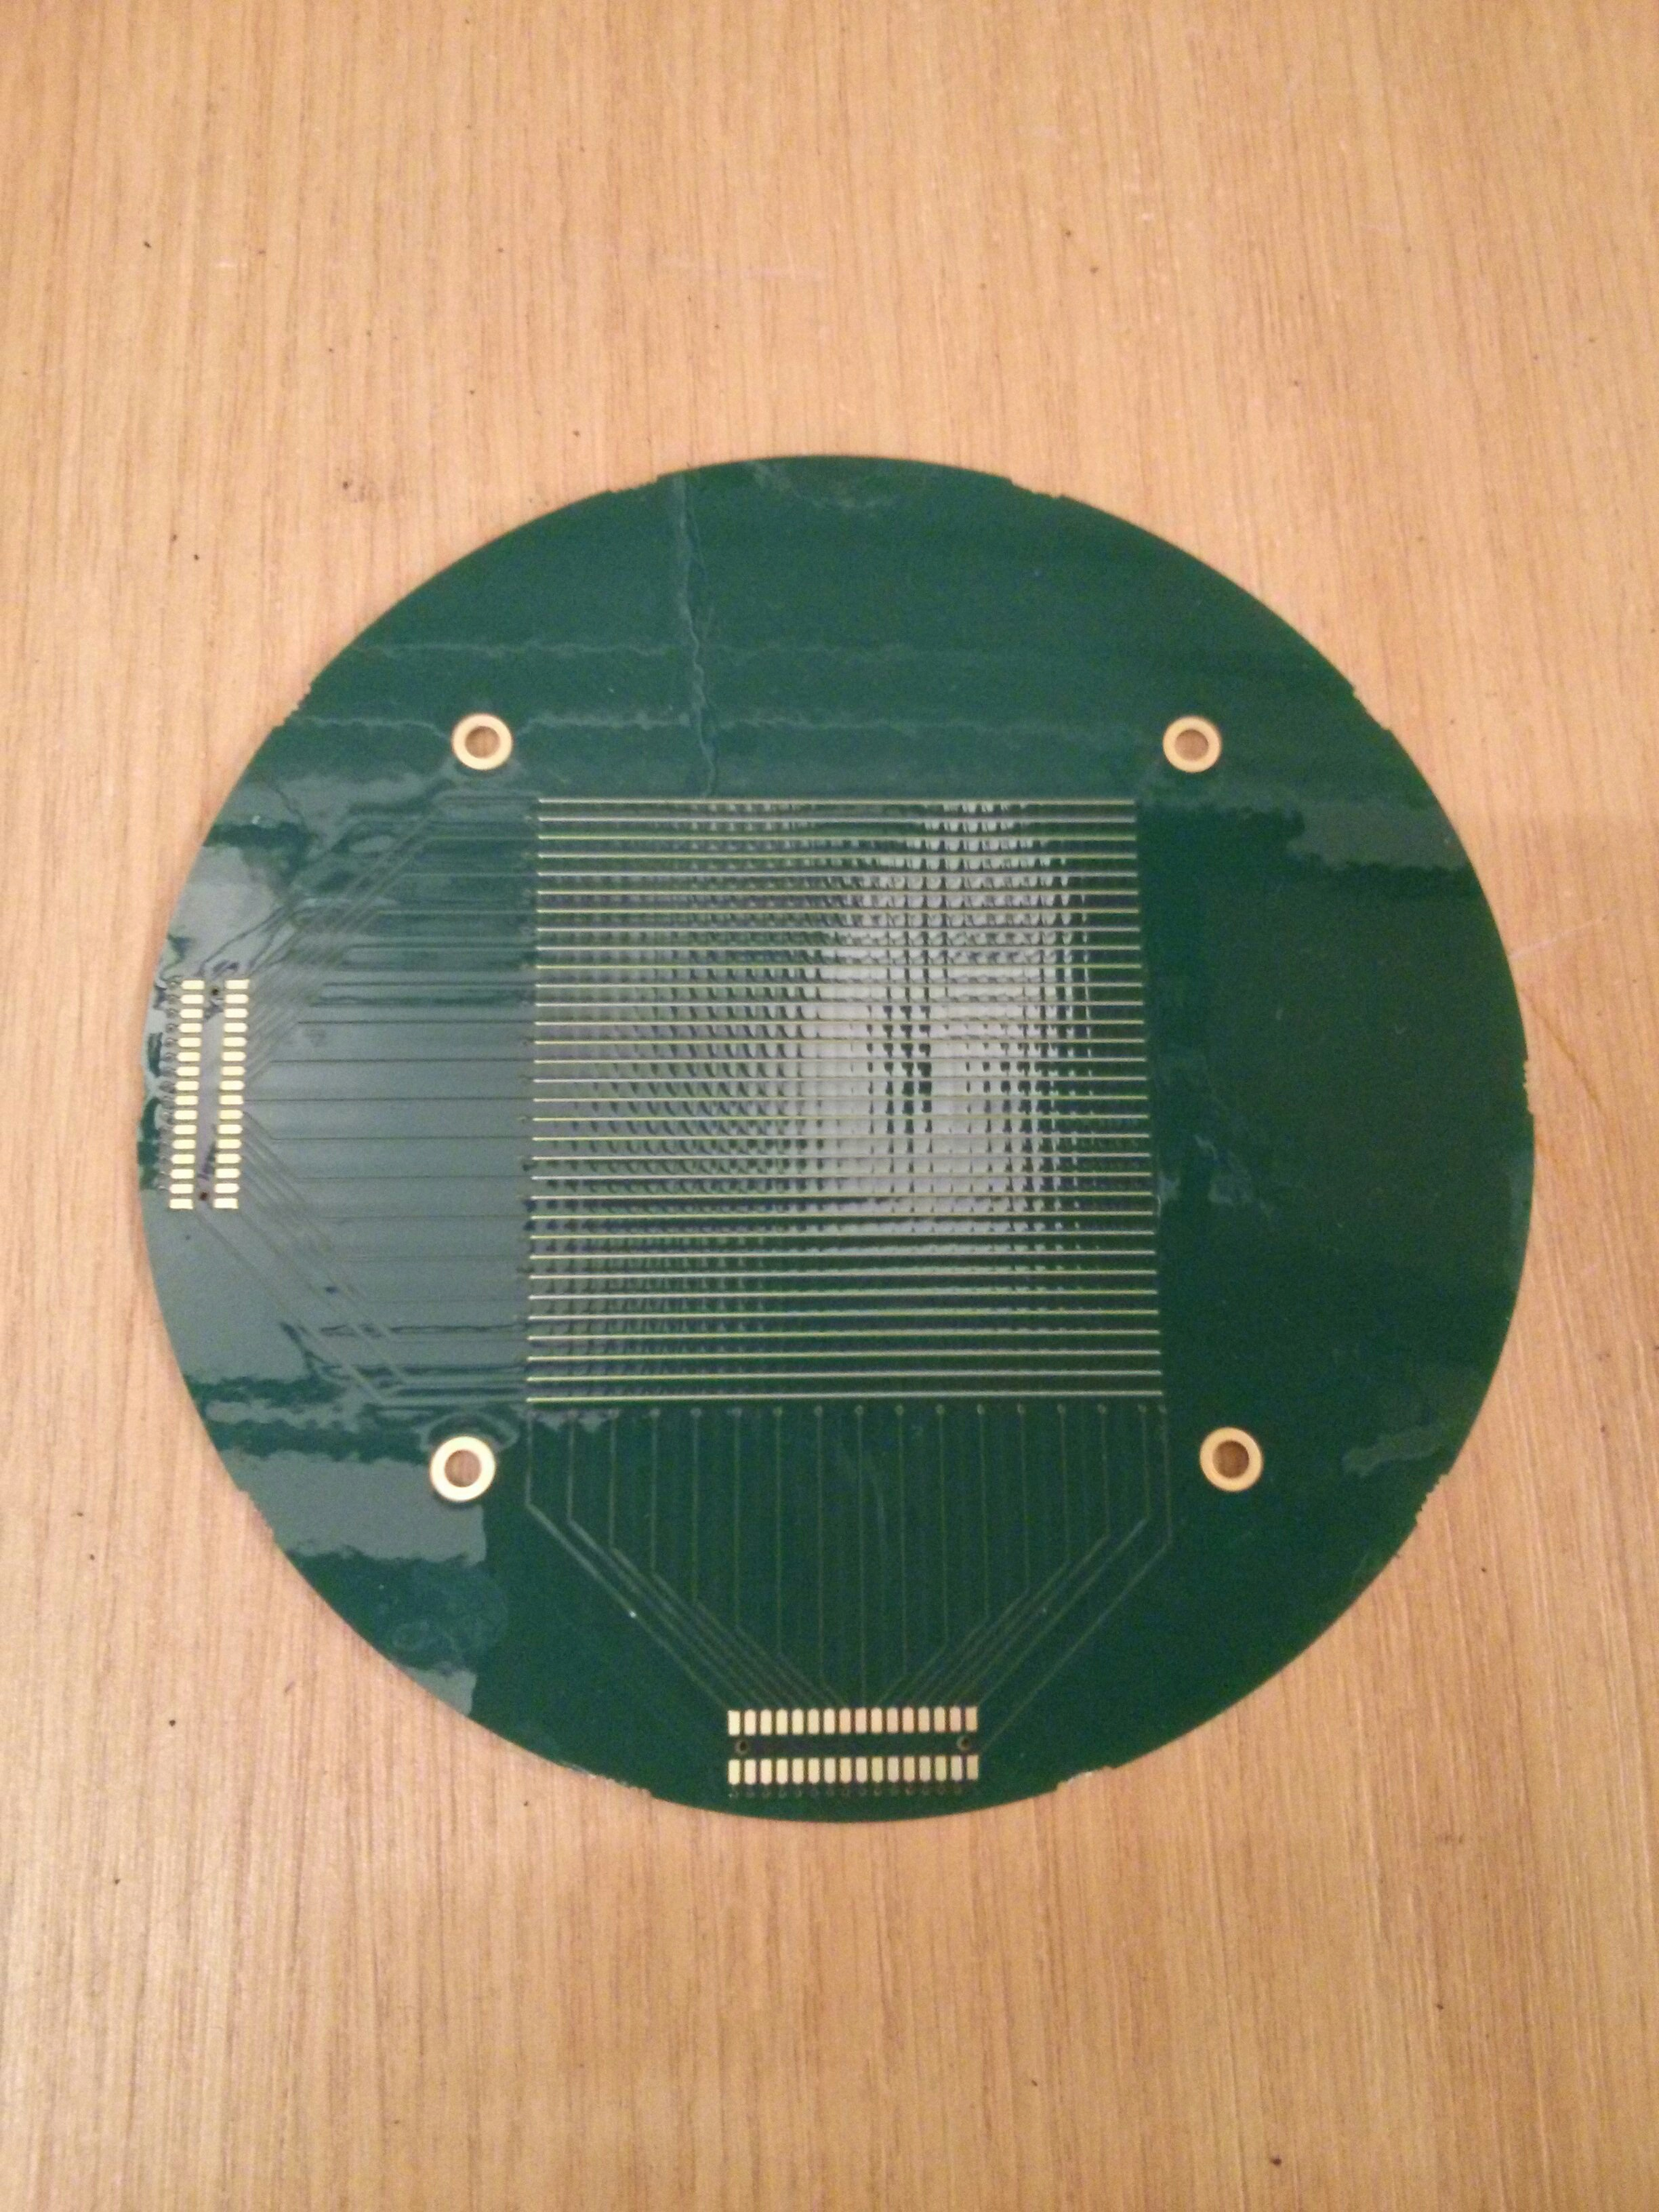
\includegraphics[width=0.5\textwidth]{cuoka/readout_plane_bottom}
	\caption{Copper on Kapton readout plane.}
	\label{fig:cuoka_readout-plane}
\end{figure}

The test was performed in a small vacuum-insulated double-batch cryostat with an inner volume of \SI{30}{\centi\metre} diameter and \SI{50}{\centi\metre} height.\todo{check dimensions}
Prior to filling, the cryostat was evacuated using a turbo-molecular pump and then purged with argon gas and evacuated a second time.
From earlier experiments~\cite{2photonAbs}, the purity can be assumed to be of the order of \SI{1}{ppb} after filling.
The cryostat is sealed using rubber o-rings which lose tightness at cryogenic temperatures.
Therefore, and due to the fact that no purification system was available, the purity degraded slowly in the course of the experiment.
The \SI{8}{\centi\metre} long field cage consists of \num{8} copper rings of \SI{8}{\centi\metre} diameter terminated by a copper plate cathode.
A field of \SI{1}{\kilo\volt\per\centi\metre} is generated using a resistive divider.

\begin{figure}[htb]
	\centering
	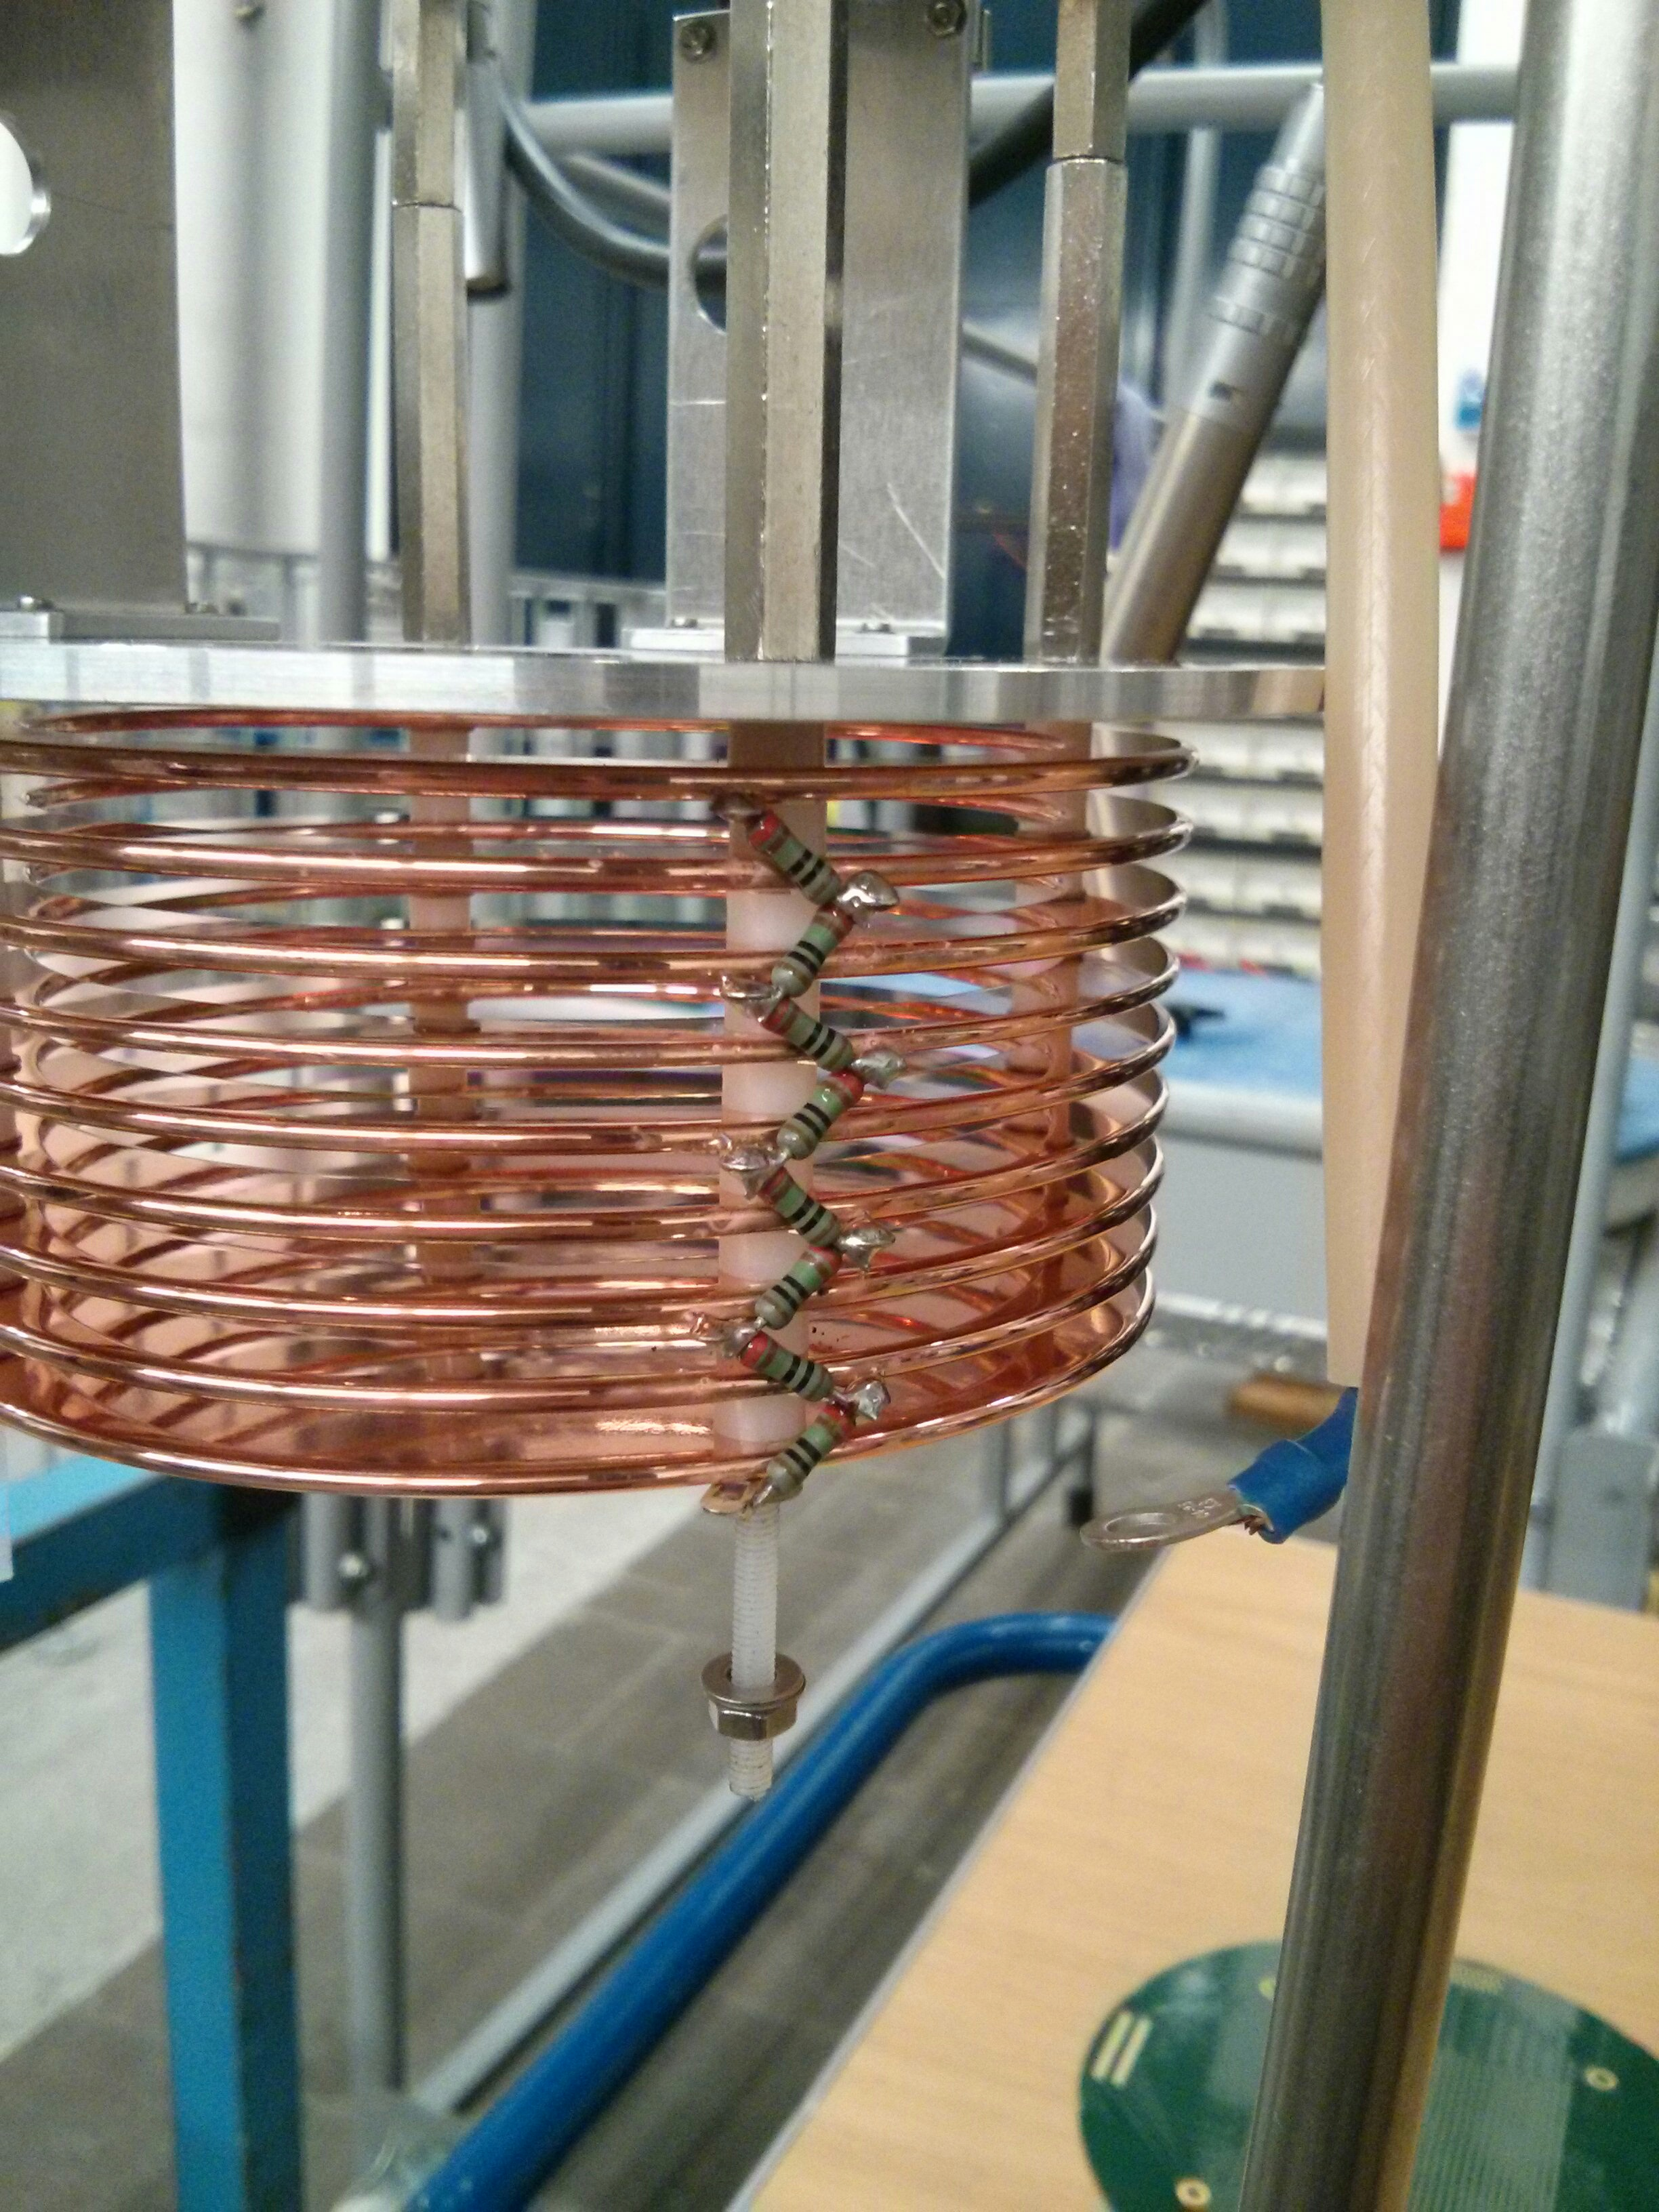
\includegraphics[width=0.5\textwidth]{cuoka/tpc}
	\caption{TPC used for the copper on Kapton readout test.}
	\label{fig:cuoka_tpc}
\end{figure}

The charge signal is amplified by cryogenic charge amplifiers.
The amplified signal is then digitised at room temperature.
The complete readout electronics chain is the one described in Section~\ref{sec:electronics_existing} before the modifications to reduce noise.

Because of the limited space inside the cryostat, no internal light triggering system could be used.
Instead, the digitisers were either triggered on one of the charge collection channels or by an external muon telescope.
The latter was formed of two scintillator panels with photomultiplier tubes above and below the crystat, respectively.
Triggering directly on charge collection channels has the potential disadvantage of recording events only partially.
If the triggering channel does not receive the first charge pulse of the event, all earlier pulses are lost, unless the data acquisition (DAQ) implements a pretrigger ring buffer of sufficient size.
It is therefore preferable to trigger on the external muon telescope.


\subsection*{Experimental Results}

Using the above-described setup, cosmic muons were recorded over the course of multiple hours.
A typical event is depicted in Figure~\ref{fig:cuoka_event}.
It can be seen that due to the event being almost parallel to the induction strips, the induction signal is in fact stronger than the collection signal.
The reason for the bad signal to noise ratio is improper grounding of the setup and high noise levels in the lab from the nearby train station and air conditioning.
Due to time constraints and an upcoming test of a pixelated readout described in Chapter~\ref{chap:dune-nd}, no analysis was performed on this data.
Anyhow, the fact that cosmic muons could be seen using this setup proves that there is no inherent problem with having the induction plane a few \SI{10}{\micro\metre} behind the collection plane.

\begin{figure}[htb]
	\centering
	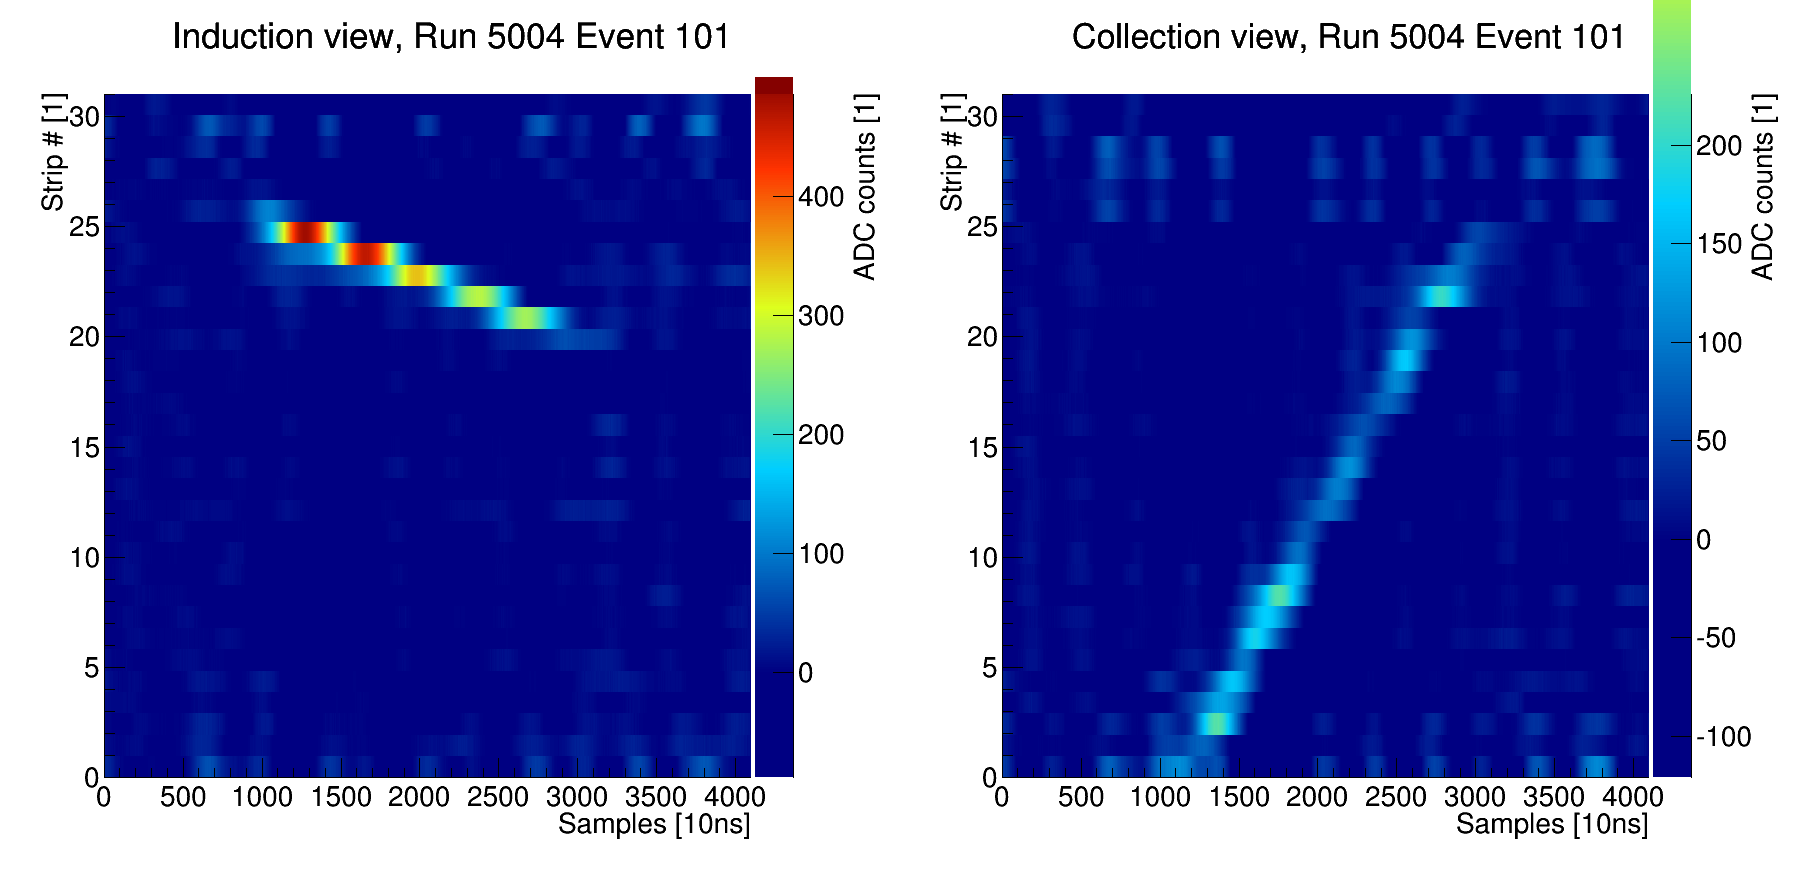
\includegraphics[width=\textwidth]{cuoka/muon_event}
	\caption{Muon event recorded using the copper on Kapton readout.}
	\label{fig:cuoka_event}
\end{figure}

While this technique can potentially solve the mechanical problems of classical wire readouts, it does not reduce the ambiguities inherent to 2D-projective readouts outlined in Section~\ref{sec:lartpc_challenges}.
Because of this, it was decided not to further investigate copper on Kapton readouts and instead focus on pixelated readouts for \lartpc{}s providing real 3D data.


\section{Pixel Readout}
\label{sec:charge-ro_pixels}

As outlined in Section~\ref{sec:lartpc_challenges}, wire readouts are not suitable for \lartpc{}s the size of the envisioned future neutrino detectors.
The ambiguities caused by the nature of wire readouts can be eliminated by using a fully pixelated readout.
Such a readout will record a true 2D image of the charge for every time slice and thus directly produce 3D space points of the event.
On the other hand, this will increase the required number of DAQ channels and therefore the data throughput.
To illustrate this, let us imagine a readout plane of \SI{1 x 1}{\metre} and a desired resolution of \SI{5}{\milli\metre}.
For a conventional wire readout with two planes, this results in

\begin{IEEEeqnarray}{rCl}
	\qty(\frac{\SI{1}{\metre}}{\SI{5}{\milli\metre}}) \times 2 & = & 40
\end{IEEEeqnarray}

wires and thus DAQ channels.
In order to reduce ambiguities, one can use more than two planes which will increase the number of channels linearly with the number of planes.
For a pixelated readout,

\begin{IEEEeqnarray}{rCl}
	\qty(\frac{\SI{1}{\metre}}{\SI{5}{\milli\metre}}) ^ 2 & = & 400
\end{IEEEeqnarray}

DAQ channels are required.
Scaling this up to the needed detector size, this leads to an enormous number of DAQ channels and data throughput.

It is possible to reduce the number of channel by employing some form of multiplexing.
There are multiple options, one could imagine for this:
\begin{itemize}
	\item Digital multiplexing
	\item Genetic multiplexing
	\item Regions of interest
\end{itemize}

Digital multiplexing means digitising all channels as close as possible to the readout plane and then mutliplexing the digital data onto a high-speed digital link.
An advantage of this technique is that the technology for this already exists and is well established in information technology.
Ideally, one would feed the data stream into an optical fibre which additionally would provide galvanic isolation of the readout from the DAQ.
The challenging part is that all of this needs to happen at cryogenic temperatures which is far from trivial because most off-the-shelf components are not made for this.
A detailed description of upcoming electronics capable of cold digitisation an multiplexing is given in Chapter~\ref{chap:electronics}.
In contrast, genetic multiplexing and regions of interest are forms of analogue multiplexing.
The difference to digital multiplexing is that multiple readout channels are combined into a single analogue link before digitising them at room temperature outside the cryostat.
In the two schemes described here, this happens by connecting multiple readout channels to a single DAQ channel.

In genetic multiplexing, the connections are done in a way that a certain event type (a single straight track for instance) forms a distinct pattern of DAQ channels activated.
For simple events, it is possible to recover the full event from the pattern.
Naturally, this reintroduces new ambiguities.
Depending on the complexity of the event topology and the degree of multiplexing, they can potentially be resolved during reconstruction.
In any case, if the event is too complex, it cannot be reconstructed properly.
While genetic multiplexing has been shown to work for one-dimensional readouts (wires), there is no known solution for two dimensions (pixels).\todo{sauce}

A third technique is to subdivide a pixelated readout plane in so-called regions of interest or ROIs.
This scheme was tested for an earlier PhD thesis at LHEP at the University of Bern using Micromegas in a xenon gas TPC~\cite{maplesyrup}.
All pixels at the same position inside the ROIs are connected to the same DAQ channel.
For instance, let us assume squared regions of interest.
One DAQ channel would connect to all the pixels in the top left corners of the ROIs.
Another channel would connect to all the pixels in the top right corner and so on.
To explain this a little better, let us assume a square pixel plane of $N \times N$ pixels where $N = n ^ 2$ with an arbitrary integer $n$.
Now, we divide the plane into $n \times n = N$, each consisting again of $n \times n = N$ pixels.
For such a readout, we require $N$ DAQ channels for the ROIs and another $N$ channels for the pixels.
We need only as many pixel channels as we have pixels per ROI because all the pixels at the same relative position inside the ROIs are connected together to one DAQ channel.
This means that we can read out a $N \times N$ pixel plane using only $2 N$ DAQ channels; the same number required by a conventional 2-plane wire readout of the same size and pitch.
If there is a signal on a certain DAQ channel, the position inside the ROI is known but not the ROI.
To determine the full position, each ROI has its own inductive grid in between the pixels.
The grid is biased such that the charge is fully focussed onto the pixels and does not collect any charge.
Combining the bipolar pulse on the ROI grid with the collection pulse from the pixels, it is possible to disentangle the true position.
Again, the drawback of this approach is that it is not free of ambiguities.
It fails for multiple simultaneous hits when it is impossible to say which pixel pulse belongs to which ROI pulse.

Independently of the amount of data one needs to bring out of the detector, a second problem is heat dissipation.
The more of the readout chain is sitting inside of the detector, the more serious this problem becomes.
It is especially problematic for digital multiplexing which requires a lot of cryogenic electronics.
A possible solution to this is to power only that part of the readout that is actually needed.
This would require a means to wake up the part of the readout where the charge is arriving before it is collected.
Provided, the wake-up time is short enough, inductive grids on regions of interest could allow precisely for this.

As the ROI approach had already been demonstrated in a gas TPC, it was chosen for the first prototype of a pixelated \lartpc{}.
Because the detector is a single-phase \lartpc{}, and thus no gas amplification as in Micromegas is needed, the readout plane could be realised as a conventional Printed Circuit Board PCB.
Alongside the PCB, a new TPC was designed which can be reused for future prototyping efforts.
The design of PCB and TPC as well as the results from the first tests are described in Chapter~\ref{chap:viper}.